\subsection{Partes} \label{subsec:partes} 

Para la construcción del brazo robótico se utilizaron motores y eslabones adecuados para soportar el peso del sistema y generar el movimiento requerido.

\textbf{Motores:} Se utilizaron dos tipos de actuadores principales:

\begin{itemize}
	\item \textbf{Motor DC MAXON RE40 con reductor planetario 100:1.} Este motor es compacto y robusto, ideal para aplicaciones de robótica que requieren alto torque y control preciso. Según su hoja de datos, puede entregar un torque continuo de hasta 63.6 mNm (antes del reductor), y su reductor planetario amplifica este torque en una proporción 100:1. Su velocidad máxima sin carga ronda los 8,000 rpm (que se reducen a 80 rpm tras el reductor), con una masa aproximada de 470 g. Este tipo de motor se empleó en articulaciones donde se requiere mayor velocidad y moderado torque.
	\begin{figure}[H]
		\centering
		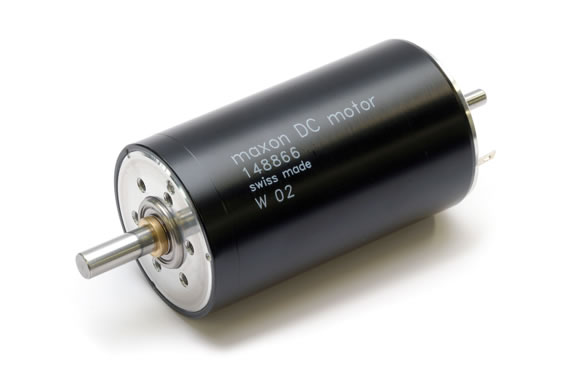
\includegraphics[width=0.4\textwidth]{motor1}
		\caption{Imagen del motor utilizado en el proyecto.}
		\label{fig:motor1}
	\end{figure}
	
	
	\item \textbf{Harmonic Drive FHA-C Mini Series, modelo FHA-25C-50-E250.} Este tipo de actuador integra motor, reductor armónico y encoder en un solo conjunto compacto. Ofrece una excelente precisión y bajo juego mecánico. El modelo FHA-25C-50-E250 tiene una relación de reducción de 50:1, un torque nominal de hasta 21 Nm y una resolución de encoder de hasta 250,000 pulsos por revolución. Se utilizó en articulaciones que requieren mayor precisión y torque constante.
	
		\begin{figure}[H]
		\centering
		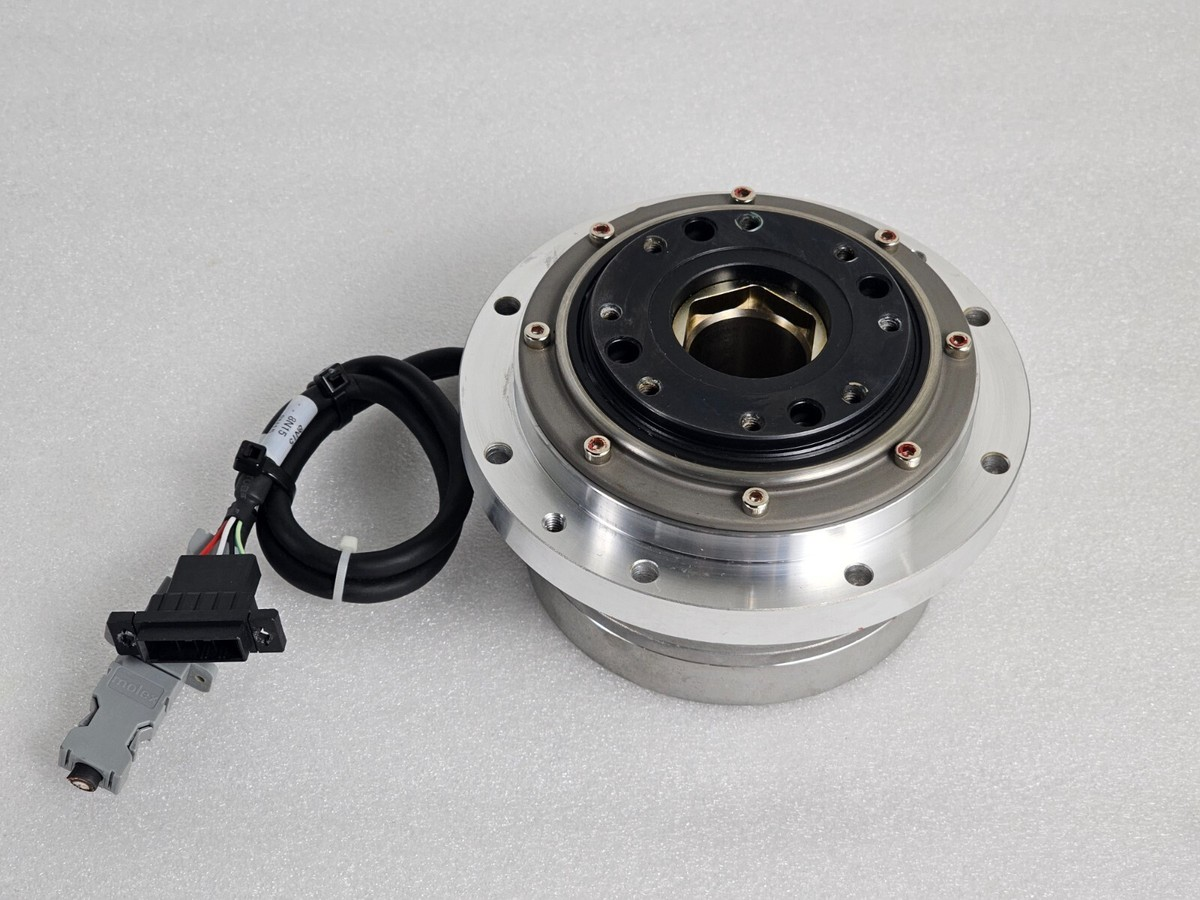
\includegraphics[width=0.4\textwidth]{motor2}
		\caption{Imagen del motor utilizado en el proyecto.}
		\label{fig:motor2}
	\end{figure}
\end{itemize}

Los torques máximos aplicados por cada articulación del brazo robótico son los siguientes:

\begin{itemize}
	\item \textbf{Articulación 1 (T1):} 0.694 Nm
	\item \textbf{Articulación 2 (T2):} 1.54 Nm
	\item \textbf{Articulación 3 (T3):} 1.33 Nm
	\item \textbf{Articulación 4 (T4):} 0.405 Nm
\end{itemize}

\textbf{Eslabones:} Todos los eslabones están fabricados en aluminio debido a su ligereza, resistencia y facilidad de mecanizado. A continuación, se describen las características de cada uno:

\begin{itemize}
	\item \textbf{Eslabón 1:} Masa de 770 g y longitud de 50 mm.
	\item \textbf{Eslabón 2:} Masa de 429 g y longitud de 152.75 mm.
	\item \textbf{Eslabón 3:} Masa de 762 g y longitud de 167 mm.
	\item \textbf{Eslabón 4:} Masa de 187 g y longitud de 95 mm.
\end{itemize}


